\section{Home Assistant}
Home Assistant je svobodný software (licence Apache) pro domácí automatizaci se
zaměřením na soukromí. Uživatel jej provozuje na vlastním serveru (například
NAS či jednodeskový počítač Raspberry Pi). Cílem projektu je
\emph{automatizace}, ne vzdálené
ovládání\footnote{\url{https://www.home-assistant.io/blog/2016/01/19/perfect-home-automation/}},
ke kterému ho lze využít také, v obvyklých situacích je ale hodnota získaná
možností ovládat různá zařízení z mobilního telefonu přinejmenším sporná.

\subsection{Instalace}
Software Home Assistant je napsaný v jazyce Python, existuje tedy několik
způsobů, jak jej nainstalovat. Nejjednodušší a pravděpodobně nejrobustnější
možností je instalace v kontejneru nástroje Docker. Podrobnou dokumentaci
s návodem pro instalaci lze nalézt na webových stránkách
\url{https://www.home-assistant.io/installation/}.
V prostředí operačního systému Debian 10 (buster) na Raspberry Pi 4 byla
instalace provedena následujícím způsobem:
\begin{lstlisting}[language=mybash]
# Stáhneme instalační skript dockeru.
cd ~/temp/ || mkdir ~/temp && cd ~/temp || exit 1
curl -fsSL https://get.docker.com -o get-docker.sh
# Jde o spustitelný soubor stažený z Internetu,
# je tedy nutné zkontrolovat jeho obsah a přesvědčit se,
# že není škodlivý.
less get-docker.sh
# Provedeme instalaci jako uživatel root.
sudo sh get-docker.sh

# Vytvoříme uživatele homeassistant a přidáme mu práva pro práci
# s dockerem.
sudo useradd -rm homeassistant -G docker
# Vytvoříme funkci umožňující snadné spouštění příkazů pod tímto
# uživatelem.
hau(){
    sudo -u homeassistant "$@"
}

hau mkdir /home/homeassistant/hass-config

# Stáhneme a spustíme vlastní kontejner.
hau docker run -d \
    --name homeassistant \
    --restart=unless-stopped \
    -e TZ=Europe/Prague \
    -v /home/homeassistant/hass-config:/config \
    --network=host \
    --privileged \
    "ghcr.io/home-assistant/home-assistant:stable"
\end{lstlisting}

Nová verze Home Assistant je vydávána každý měsíc (například verze 2022.3.0
v březnu roku 2022), v průběhu měsíce jsou navíc vydávány opravné verze
(2022.3.1; 2022.3.2 atd.). V době psaní tohoto textu je nejnovější stabilní
verze 2022.3.2.
Proces aktualizace je poměrně jednoduchý, obsahuje ale několik kroků:
\begin{enumerate}[nosep]
    \item (volitelně) odstranění starých verzí kontejneru pro úsporu místa na
        systémovém disku,

    \item stažení nového image kontejneru příkazem \shellcmd{docker pull},

    \item zastavení starého kontejneru (\shellcmd{docker stop homeassistant}),

    \item odstranění starého kontejneru (\shellcmd{docker rm homeassistant}),

    \item (volitelně) záloha konfiguračních souborů a databáze,

    \item spuštění nového kontejneru příkazem \shellcmd{docker run} se stejnými
        přepínači jako při instalaci.
\end{enumerate}
U procesů s vícero netriviálními kroky strmě narůstá riziko lidské chyby,
proto byl vytvořen jednoduchý skript, který postup aktualizace automatizuje.
Jeho zdrojový kód je otištěn v příloze~\vref{app:update ha}.

Po spuštění poslouchá webový server Home Assistant na portu \port{8123/tcp}.
Pokud je na serveru provozován firewall, je nutné tento port otevřít pro
zařízení, která mají mít k webovému rozhraní přístup. S jednoduchým nástrojem
pro konfiguraci \shellcmd{iptables} nazvaným \shellcmd{ufw}
(\foreignlanguage{english}{Uncomplicated FireWall} to lze provést následovně:
\begin{lstlisting}[language=mybash]
sudo tee /etc/ufw/applications.d/homeassistant << EOF
[homeassistant]
title=Home Assistant Web UI
description=Home Assistant Web UI
ports=8123/tcp
EOF
sudo ufw app update homeassistant

# Výpis informací o aplikaci:
sudo ufw app info homeassistant

# Povolení komunikace pro konkrétní zařízení:
sudo ufw allow from 192.168.1.4 to any app homeassistant comment "Home Assistant moje PC"
\end{lstlisting}


\subsection{Konfigurace}
Konfigurace Home Assistant se provádí zčásti přímo z webového rozhraní a zčásti
pomocí konfiguračních souborů ve formátu YAML. Projekt budíku komunikuje s Home
Assistant pomocí protokolu MQTT, zaměříme se proto pouze na konfiguraci pomocí
YAML souborů.

Veškerou konfiguraci by bylo možné vkládat do hlavního konfiguračního souboru
\filename{configuration.yaml}.
Z hlediska zachování přehlednosti a jednoduchosti údržby je ale vhodnější
konfiguraci rozdělit do více souborů.
Můžeme využít funkci
\texttt{packages}\footnote{\url{https://www.home-assistant.io/docs/configuration/packages/}},
která nám umožní členit konfiguraci podle libovolného kritéria (například podle
fyzického zařízení). Běžná metoda využívající
\lstinline[language=yaml]|!include nazev_souboru.yaml| totiž umožňuje pouze
členění podle domény (\HAdomain{sensor}, \HAdomain{binary_sensor},
\HAdomain{light}, ...). Takto vytvoření balíček konfigurace je také vhodný pro
následnou distribuci, protože jeho použití je naprosto triviální.

V hlavním konfiguračním souboru \filename{configuration.yaml} přidáme záznam,
který určuje, že jednotlivé balíčky konfigurace se nacházejí v adresáři
\filename{packages/}.
\begin{lstlisting}[language=yaml]
homeassistant:
  packages: !include_dir_named packages
\end{lstlisting}
V tomto adresáři poté můžeme vytvořit soubor
\filename{packages/alarmclock.yaml}, který obsahuje úplnou konfiguraci všech
entit tvořících budík.
\begin{lstlisting}[language=yaml]
switch:
  - platform: mqtt
    name: AlarmClock inhibit
    state_topic: alarmclock/stat/inhibit
    command_topic: alarmclock/cmnd/inhibit
    availability_topic: alarmclock/stat/available

# ...
\end{lstlisting}


% Obecne info o HA:
% https://www.home-assistant.io/docs/glossary/
% jinja2 templates

\subsection{Integrace s budíkem}
MQTT adaptér \shellcmd{ac2mqtt} popisovaný v předchozím textu
umožňuje snadnou integraci s tímto systémem. Platforma \texttt{mqtt} nabízí
v prostředí Home Assistant možnost vytvářet entity z celé řady domén~--
například \HAdomain{sensor}, \HAdomain{binary_sensor}, \HAdomain{light},
\HAdomain{switch} a další.

Příkladem funkce budíku, kterou lze do systému snadno integrovat, je ovládání
světla \uv{lamp}. To je určeno primárně pro buzení, není ale důvod, proč by
nemohlo být využíváno i pro jiné účely. Protože jde o osvětlení, využijeme typ
entity
\href{https://www.home-assistant.io/integrations/light.mqtt}{MQTT Light}.
Vlastní konfigurace je triviální:
\begin{lstlisting}[language=yaml]
light:
  - platform: mqtt
    name: AlarmClock lamp
    state_topic: alarmclock/stat/lamp
    command_topic: alarmclock/cmnd/lamp
    availability_topic: alarmclock/stat/available
\end{lstlisting}
Využíváme výchozích hodnot~-- například \lstinline!payload_off: OFF!
a~\lstinline!payload_on: ON!. Ty se shodují se zprávami odesílanými programem
\shellcmd{ac2mqtt}. \yamlkey{availability_topic} složí k detekci
nefunkčního spojení s budíkem. V takovém případě přejde entita
\HAentity{light.alarmclock_lamp} do stavu \HAstate{unavailable}.

Platforma \foreignlanguage{english}{MQTT Light} umožňuje i ovládání jasu
světla, čehož využíváme u stmívatelné LED \uv{ambient}. Konfigurace je
o něco složitější.
\begin{lstlisting}[language=yaml]
light:
  - platform: mqtt
    schema: template
    name: AlarmClock ambient
    availability_topic: alarmclock/stat/available
    command_topic: alarmclock/cmnd/ambient
    state_topic: alarmclock/stat/ambient
    state_template: "{{ 'off' if value == '0' else 'on' }}"
    brightness_template: "{{ value }}"
    command_off_template: 0
    command_on_template: >
      
      {{ brightness }}
      
      255
      
\end{lstlisting}
Protože je LED pásek řízen pouze jasem, kde hodnota \num{255} představuje plný
jas a \num{0} představuje zhasnuté světlo, je stav entity (zapnuto / vypnuto)
z tohoto čísla. To je úlohou šablony \yamlkey{state_template}. Protože proměnná
\texttt{value} představuje textový řetězec přijatý na \yamlkey{state_topic},
porovnáváme ji s textovým řetězcem \lstinline[language=Python]!'0'!. Druhou
možností by bylo převést \texttt{value} na celočíselný datový typ filtrem
\texttt{int} a porovnávat čísla.

\yamlkey{brightness_template} určuje, jak z přijaté MQTT zprávy odvodit jas
světla jako číslo v rozsahu \numrange{0}{255}.

\yamlkey{command_off_template} specifikuje zprávu, která se má poslat na
\yamlkey{command_topic}, když je požadováno vypnutí světla. Protože vypnutí
provádíme nastavením jasu na \num{0}, není ani potřeba využít šablonu.

\yamlkey{command_on_template} je složitější, protože musí správně reagovat
v různých situacích:
\begin{enumerate}[nosep]
    \item Je požadováno zapnutí světla, ale není specifikován jas. V takovém
        případě není proměnná \texttt{brightness} definována a do
        \yamlkey{command_topic} se pošle hodnota \num{255}.
    \item Je požadované zapnutí světla s určitou hodnotou jasu. V takovém
        případě se v~MQTT zprávě pošle hodnota proměnné \texttt{brightness}.
\end{enumerate}

\begin{figure}[htb]
    \centering
    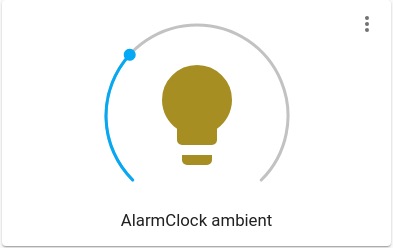
\includegraphics[width=0.3\textwidth]{homeassistant-lovelace-light}
    \caption{%
        Karta \href{https://www.home-assistant.io/lovelace/light/}{Light}
        reprezentující entitu \HAentity{light.alarmclock_ambient} v prostředí
        Lovelace systému Home Assistant
    }
    \label{fig:homeassistant lovelace light}
\end{figure}

Úplný balíček konfigurace pro Home Assistant je otištěn
v příloze~\vref{app:HAconfig}.


\subsubsection{Recorder}
Ve výchozí konfiguraci je přidána integrace \HAintegration{recorder}. Ta
automaticky nahrává historii stavu všech entit, přičemž data jsou ukládána do
SQL databáze. Integrace \HAintegration{history} umožňuje tato historická data
procházet a tvořit z nich grafy. Integrace \HAintegration{logbook} zobrazuje
tato data ve formě textových, chronologicky řazených popisů událostí.

\begin{figure}[htb]
    \centering
    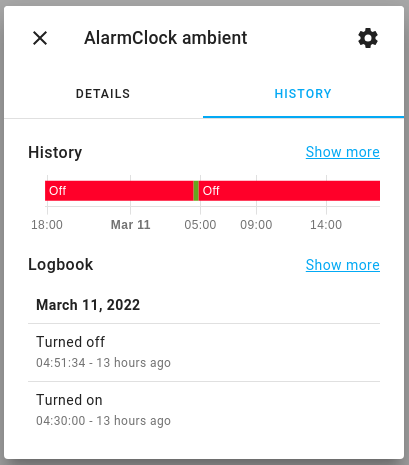
\includegraphics[width=0.5\textwidth]{homeassistant-history}
    \caption{%
        Graf \HAintegration{history} a výpis \HAintegration{logbook} v~detailu
        entity \HAentity{light.alarmclock_ambient}
    }
    \label{fig:homeassistant lovelace light history}
\end{figure}
